\documentclass[a4paper,UTF8]{article}
\usepackage{ctex}
\usepackage[margin=1.25in]{geometry}
\usepackage{color}
\usepackage{graphicx}
\usepackage{amssymb}
\usepackage{amsmath}
\usepackage{amsthm}
\usepackage{bm}
\usepackage{hyperref}
\numberwithin{equation}{section}
%\usepackage[thmmarks, amsmath, thref]{ntheorem}
\theoremstyle{definition}
\newtheorem*{solution}{Solution}
\newtheorem*{prove}{Proof}
\usepackage{multirow}

%--

%--
\begin{document}
\title{机器学习导论\\
习题三}
\author{学号, 作者姓名, 邮箱}
\maketitle
\section{[30pts] Decision Tree Analysis}
决策树是一类常见的机器学习方法,但是在训练过程中会遇到一些问题。

(1) \textbf{[10pts]} 试证明对于不含冲突数据(即特征向量完全相同但标记不同)的训练集,必存在与训练集一致(即训练误差为0)的决策树;

(2) \textbf{[10pts]} 试分析使用“最小训练误差”作为决策树划分选择的缺陷。
\begin{solution}
此处用于写证明(中英文均可)\\
(1)假设不存在与训练集一致的决策树,则必然存在一棵决策树,它的某个叶子节点上有两个标记不同的示例。因为该叶子节点无法继续划分,所以,这两个标记不同的示例必然有相同的特征向量,这就和训练集中不含冲突数据矛盾。\\
(2)使用最小训练误差,会使得决策树过拟合,从而泛化能力降低。
\end{solution}

\section{[30pts] Training a Decision Tree}
考虑下面的训练集:共计6个训练样本,每个训练样本有三个维度的特征属性和标记信息。详细信息如表\ref{table:training}所示。

请通过训练集中的数据训练一棵决策树,要求通过“信息增益”(information gain)为准则来选择划分属性。请参考书中图4.4,给出详细的计算过程并画出最终的决策树。
\begin{table}[h]
\centering
\caption{训练集信息}
\label{table:training}\vspace{2mm} 
\begin{tabular}{c|c c c|c}\hline
序号		&  特征 \textbf{A} 	&	特征 \textbf{B}	&	特征 \textbf{C} 	&	标记    \\ \hline
1		&  0 	&	1	&	1 	&	0    \\
2		&  1 	&	1 	&	1 	&	0    \\
3		&  0 	&	0 	&	0 	&	0    \\
4		&  1 	&	1 	&	0 	&	1    \\
5		&  0 	&	1 	&	0 	&	1    \\
6		&  1 	&	0 	&	1 	&	1    \\\hline
\end{tabular} 
\end{table}

\begin{solution}
此处用于写解答(中英文均可)\\
$Ent(D)=-\sum_{k=1}^2 p_k log_2 p_k = - (\frac{1}{2} log_2 \frac{1}{2} + \frac{1}{2} log_2 \frac{1}{2}) = 1$\\
$Ent(D^0_A) = -(\frac{1}{3} log_2 \frac{1}{3} + \frac{2}{3} log_2 \frac{2}{3}) = 0.918$,$Ent(D^1_A) = -(\frac{1}{3} log_2 \frac{1}{3} + \frac{2}{3} log_2 \frac{2}{3}) = 0.918$\\
$Gain(D,A) = Ent(D) - \sum_v\frac{\vert D^v_A \vert}{\vert D \vert} Ent(D^v_A)=0.082$\\
$Ent(D^0_B) = -(\frac{1}{2} log_2 \frac{1}{2} + \frac{1}{2} log_2 \frac{1}{2}) = 1$,$Ent(D^1_B) = -(\frac{2}{4} log_2 \frac{2}{4} + \frac{2}{4} log_2 \frac{2}{4}) = 1$\\
$Gain(D,B) = Ent(D) - \sum_v\frac{\vert D^v_B \vert}{\vert D \vert} Ent(D^v_B)=0$\\
$Ent(D^0_C) = -(\frac{1}{3} log_2 \frac{1}{3} + \frac{2}{3} log_2 \frac{2}{3}) = 0.918$,$Ent(D^1_C) = -(\frac{1}{3} log_2 \frac{1}{3} + \frac{2}{3} log_2 \frac{2}{3}) = 0.918$\\
$Gain(D,C) = Ent(D) - \sum_v\frac{\vert D^v_C \vert}{\vert D \vert} Ent(D^v_C)=0.082$\\
在A和C属性上均取得最大信息增益,选取A作为划分属性。\\
生成两个子节点:D1={1,3,5},D2={2,4,6}\\
$Ent(D1)=0.918$\\
$Ent(D1^0_B) = 0$,$Ent(D1^1_B) = 1$\\
$Gain(D1,B)=0.918-(\frac{1}{3} 0 + \frac{2}{3} 1) = 0.251$\\
$Ent(D1^0_C) = 1$,$Ent(D1^1_C) = 0$\\
$Gain(D1,C)=0.251$\\
在B和C属性上均取得最大信息增益,选取B作为划分属性。\\
生成两个子节点:D11={3},D12={1,5}。其中,D11不需要再划分,D12按照C属性的取值,可以再次划分为两个子节点:D121={5},D122={1}。\\
$Ent(D2)=0.918$\\
$Ent(D2^0_B) = 0$,$Ent(D2^1_B)=1$\\
$Gain(D2,B)=0.251$\\
$Ent(D2^0_C) = 0$,$Ent(D2^1_C)=1$\\
$Gain(D2,C)=0.251$\\
在B和C属性上均取得最大信息增益,选取B作为划分属性。\\
生成两个子节点:D21={6},D22={2,4}。其中,D21不需要再划分,D22按照C属性的取值,可以再次划分为两个子节点:D221={2},D222={4}。\\
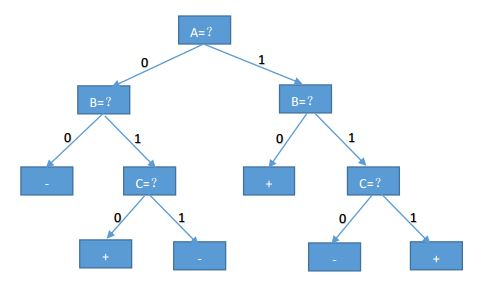
\includegraphics[height=8cm]{a.jpg}
\end{solution}

\section{[40pts] Back Propagation} 
单隐层前馈神经网络的误差逆传播(error BackPropagation,简称BP)算法是实际工程实践中非常重要的基础,也是理解神经网络的关键。

请编程实现BP算法,算法流程如课本图5.8所示。详细编程题指南请参见链接:\url{http://lamda.nju.edu.cn/ml2017/PS3/ML3_programming.html}

在实现之后,你对BP算法有什么新的认识吗?请简要谈谈。
\begin{solution}
此处用于写解答(中英文均可)\\
我原来错误地以为如果一个样例的标号为3,那么它的10个输出值当中,第三个数必定会逼近1,其余的9个数都逼近0,但是实际上并不是。这10个预测值可以是任意的,只要满足第三位的值比其他几个值大,就可以正确分类了。这点是我有点没明白的。\\
另外就是,我一开始将调整的值的符号写错了,全部都是加(书上是权重加,阈值减),然而貌似并不会特别影响整个模型,模型似乎任然可以正确预测,并有较高的精度。我觉得应该是模型可以主动纠正,所以符号的正负并不会有什么影响。
\end{solution}

\section*{附加题   [30pts] Neural Network in Practice}
在实际工程实现中,通常我们会使用已有的开源库,这样会减少搭建原有模块的时间。因此,请使用现有神经网络库,编程实现更复杂的神经网络。详细编程题指南请参见链接:\url{http://lamda.nju.edu.cn/ml2017/PS3/ML3_programming.html}

和上一题相比,模型性能有变化吗?如果有,你认为可能是什么原因。同时,在实践过程中你遇到了什么问题,是如何解决的?
\begin{solution}
此处用于写解答(中英文均可)\\
模型的预测准确度更高了。同样迭代次数(100次),大概高2到3个百分点。\\
我认为性能提高可能是由于模型训练中使用的优化函数的区别。这一题的优化器是Adam,而不是SGD。
\end{solution}



\end{document}